%%%%%%%%%%%%%%%%%%%%%%%%%%%%%%%%%%%%%%%%%%%%%%%%%%%%%%%%%%%%%%%%%%%%%%%%%%%%%%%%%%%%%%%%%%%
\section{Discussion}\label{sec:discussion}

\subsection{Solution}\label{sec:solution}

The solution to the differential equation \eqref{eq:susyConditionTheta} is:
\begin{equation}\label{eq:susyConditionSolution}
\boxed{\sin\theta(c) = L \sqrt{c^2-1}; \quad 1 < c \leq \sqrt{1+L^{-2}}},
\end{equation}
where $L$ is an integration constant. As we will show below, it is the asymptotic separation of the D7-brane from the stack of the D3-branes, in the units of the spherical radius\footnote{The spherical part of our metric \eqref{eq:PWmetric} is multiplied by $R^2$.} $R$, namely $L$ above is really $ L/R$.
We have set $R=1$ so far. The upper bound of $c$ is set by the maximum of the sine.


Near the boundary, $c \approx 1 + z^2/2$, the solution behaves as
\begin{equation} \label{eq:thetaExpanded}
 \theta(z) \approx L \, z + \left(\frac{L}{8} +\frac{L^3}{6} \right) \, z^3 + O(z^5).
\end{equation} 
Moreover, keeping only the leading order of the large $L$ expansion (i.e. $L\gg R$), our solution reduces to the one found in the $AdS_5 \times S^5$ background, see \cite{Karch:2002sh} and \cite{Karch:2005ms}, i.e.
\begin{equation}
 \sin\theta(z)_\text{AdS} = L z,
\end{equation}
with the asymptotic expansion
\begin{equation}
\theta(z)_\text{AdS} \approx L z + \frac{L^3}{6} z^3 + O(z^5).
\end{equation}



As \cite{Karch:2005ms} explains, in the flat embedding space limit, this embedding describes a planar D-brane located at a constant distance $L$ away from the stack of $N$ D3-branes:
\begin{equation}
 L = \lim_{z \rightarrow 0 } \frac{R}{z} \sin\theta(z) = R \, L/R,
\end{equation}
where we explicitly stated $R$. Furthermore, this separation is proportional to the quark mass $m$:
\begin{equation}
 L = 2 \pi l_s^2 m.
\end{equation}


Figures in \ref{fig:vielbeins} show the vielbeins of the induced metric at the solution, from which we learn how the geometry of the embedding looks like at different values of $c$. First, observe the divergence at the horizon $c_{max}=\sqrt{1+L^{-2}}$. This is the location of the well-known enhançon locus, at $\theta = \pi/2$, see \cite{Buchel:2000cn} and \cite{Evans:2000ct}. The spheroid is undeformed at the boundary $c=1$, and becomes squashed until it vanishes at the enhançon. 

\begin{figure}[t!]
\begin{center}
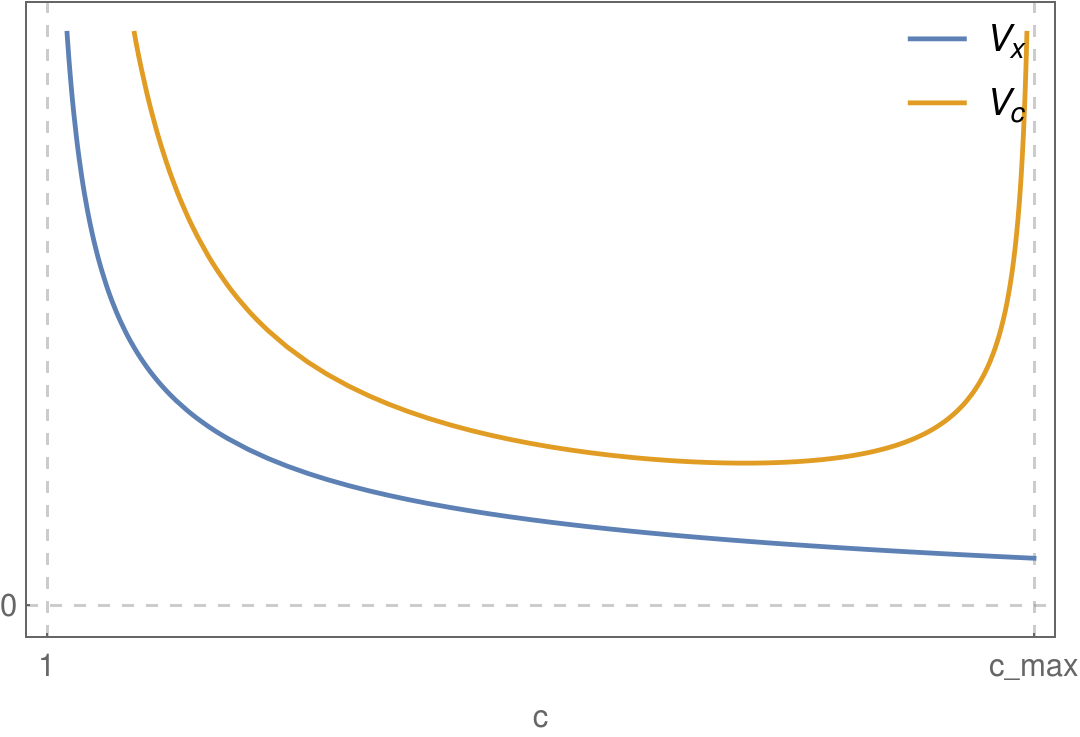
\includegraphics[width=0.6\textwidth]{pictures/vxvcb.png}
\end{center}
\vspace{0.05mm}
\begin{center}
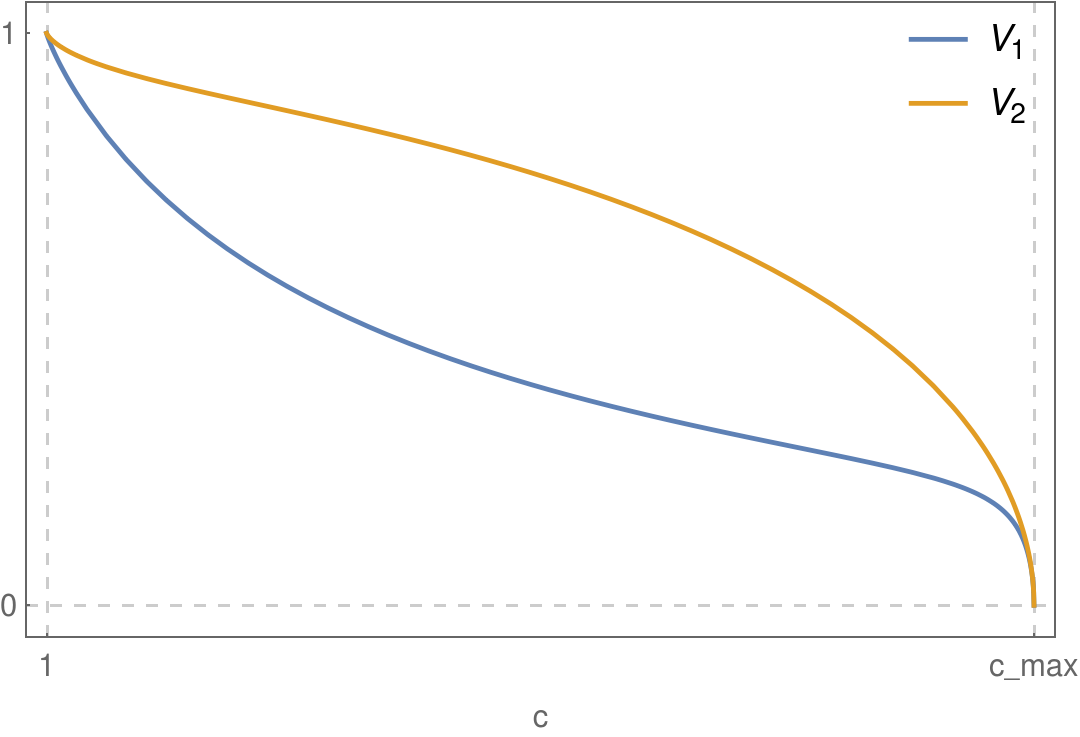
\includegraphics[width=0.6\textwidth]{pictures/v1v2b.png}
\end{center}
\caption{\label{fig:vielbeins} The vielbeins of the induced metric for the allowed values of $c$.}
\end{figure}



%%%%%%%%%%%%%%%%%%%%%%%%%%%%%%%%%%%%%%%%%%%%%%%%%%%%%%%%%%%%%%%%%%%%%%%%%%%%%%%%%%%%%%%%%%%%%%%%%
\subsection{Action}


The D7-brane action \eqref{eq:DbraneAction} for our configuration \eqref{eq:ansatz} can be written as:
\begin{align} \label{eq:ActionWithTheta'}
 S  = & -T_7 \int_\mathcal{M} d^8\xi \, e^{-P[\Phi] } v_x^4 v_c v_1 v_2^2 \sqrt{1+\frac{v_\theta^2}{v_c^2}\theta'(c)^2}  \nonumber \\
      & + T_7\int _\mathcal{M} P[C_{(8)}],
\end{align}
or more explicitly, using the solution \eqref{eq:susyConditionTheta}, as:
\begin{align}\label{eq:ActionWithTheta}
 S = & -T_7 \int_\mathcal{M} d^8\xi \, \dfrac{c A(c) \cos^3\theta (c) \sqrt{X_1(c, \theta(c))}}{\left(c^2-1\right)^3} \sqrt{1+ c A(c) \tan^2\theta(c)} \nonumber \\
     & +T_7\int _\mathcal{M} d^8\xi \, \dfrac{A(c)^2 \cos^4\theta(c)}{4 \left(c^2-1\right)^2}.
\end{align}
The explicit form of the Wess-Zumino term is calculated below.

\subsubsection{Wess-Zumino term}
The $P[C_{(8)}]$ term was deemed vanishing in \cite{Albash:2011nw} and \cite{Evans:2005ti}. Their argument did not consider the dilaton factor in the string frame that affects the Hodge star operation while deriving $C_{(8)}$, which in our scenario is
\begin{equation}
 dC_{(8)} = \ast dC_{(0)}.
\end{equation}
The dilaton term from the string frame effectively cancels the factor that vanishes at $\phi_0$, leading to a finite value for the pullback of this potential. We decided to compute it explicitly, and the full result is given in the appendix \ref{sec:backgroundFields}. We can quickly see that it is non-zero for our ansatz for $\phi$ in \eqref{eq:ansatz}. However, $P[C_{(8)}]$ term can be much simpler, as we will see now. First, we can show that:
\begin{equation}\label{eq:C8id}
 [d C_{(8)}]_{\phi_0} = d [C_{(8)}]_{\phi_0}.
\end{equation}
The left-hand-side is simply
\begin{equation}
 [d C_{(8)}]_{\phi_0}  = \dfrac{A^2 \sin\theta \cos^3(\theta)}{\left(c^2-1\right)^2} 
\sigma_1 \wedge \sigma_2 \wedge \sigma_3 \wedge dc  \wedge dx_0 \wedge dx_1 \wedge dx_2 \wedge dx_3 \wedge d\theta,
\end{equation}
and, via \eqref{eq:C8id}, we can integrate the above expression over $\theta$ and obtain:
\begin{equation}
[C_{(8)}]_{\phi_0} = \dfrac{A^2 \cos^4\theta}{4 \left(c^2-1\right)^2} \sigma_1 \wedge \sigma_2 \wedge \sigma_3 \wedge dc \wedge dx_0 \wedge dx_1 \wedge dx_2 \wedge dx_3.
\end{equation}
The full pullback is obtained by just replacing $\theta$ by $\theta(c)$.




%%%%%%%%%%%%%%%%%%%%%%%%%%%%%%%%%%%%%%%%%%%%%%%%%%%%%%%%%%%%%%%%%%%%%%%%%%%%%%%%%%%%%%%%%%%%%%%%%

\subsection{Equation of motion}

As a consistency check for our results, the equation of motion from the action \eqref{eq:ActionWithTheta'} is fulfilled with the solution \eqref{eq:susyConditionTheta}. In particular, 
\begin{align}\label{eq:eom}
-\left.EL[\mathcal{L}_{DBI}]\right|_\text{solution} = EL[\mathcal{L}_{WZ}] = \dfrac{A^2 \sin\theta \cos^3(\theta)}{\left(c^2-1\right)^2},
\end{align}
where $EL[\cdot]$ is the Euler-Lagrange operator:
\begin{equation}
 EL[\mathcal{L}] = 
 \left(\dfrac{\pd }{\pd \theta(c)} -\dfrac{\pd }{\pd c}  \dfrac{\pd }{\pd \theta'(c)} \right) \mathcal{L}.
\end{equation}
Therefore, \eqref{eq:eom} is another proof for the non-vanishing WZ term.



\subsection{Holographic renormalization}
The fully explicit on-shell action evaluated at the solution \eqref{eq:susyConditionSolution} is:
\begin{align}\label{eq:ActionAtSolution}
 S_\text{reg} = -T_7 V \int_{1 + \epsilon^2/2}^{c_\text{max}} d c \, 
 &\left[-\frac{c A(c)}{\left(c^2-1\right)^3} -\frac{A(c)^2}{4 \left(c^2-1\right)^2} \right. \nonumber\\
 &-\frac{L^2 A(c) \left(\left(c^2+1\right) A(c)-4 c\right)}{2 \left(c^2-1\right)^2} \nonumber\\
 &+\left.\frac{L^4 A(c) \left(3 c^2 A(c)+A(c)-4 c\right)}{4 \left(c^2-1\right)}\right],
\end{align}
where $c_\text{max}$ is the upper bound shown in \eqref{eq:susyConditionSolution}, and $V$ denotes the volume of the 4-dimensional Minkowski space times the 3-sphere. Notice that the action is divergent near the boundary, thus, we regularized it by adding a regulator $\epsilon>0$ in the lower integration limit. 

From the exact integrations in the appendix \ref{sec:integrate-action}, we can identify the divergent terms:
\begin{align} \label{eq:Sdiv}
 S_\text{div} = T_7 V 
        \left[ \frac{1}{4 \epsilon ^4} +\frac{1+\log \left(\epsilon/2\right)}{2 \epsilon ^2}-\frac{L^2}{2 \epsilon ^2}-\frac{ \log ^2\left(\epsilon/2\right)}{4}+\frac{\log (\epsilon )}{8} \right],
\end{align}
which come from the $L^0$ and $L^2$ terms of \eqref{eq:ActionAtSolution}. 

In holographic renormalization, the counterterms must be covariant and local on the regulator hypersurface. They do not only subtract the divergences, but also finite terms from both IR and UV, such that the final action vanishes, required by supersymmetry. For general asymptotic AdS spaces and for the D7-brane in particular, the counterterms are derived in \cite{Karch:2005ms} (we do not copy the ones with curvature below):
\begin{align} \label{eq:Ls}
& L_{1}=-\frac{1}{4} \sqrt{\gamma} \nonumber\\
& L_{4}=\frac{1}{2} \sqrt{\gamma} \theta(\epsilon)^2 \nonumber\\
& L_{f}= -\frac{5}{12}\sqrt{\gamma} \theta(\epsilon)^4,
\end{align}
where $\gamma$ here denotes the determinant of the regulator hypersurface metric. 
However, for our case, these counterterms do not apply. Our geometry is seemingly not covered by this general study, due to the logarithmic divergence appearing already at the next-to-leading order $\epsilon$-expansion for the metric, coming from $A(c)$. The explanation is that the 10-dimensional Pilch-Warner background is uplifted from the 5-dimensional supergravity solution, and indeed the logarithmic divergence mentioned comes from fields in the 5-dimensional theory, not from the 5-dimensional metric; see \cite{Bobev:2013cja}. If we were to find covariant counterterms, these woulb be written in terms of these lower dimensional fields too.


Let us be concerned for now in the counterterms that are not finite, i.e. it cancels exactly $S_\text{div}$. We propose:
\begin{equation}\label{eq:counterterms}
 S_\text{CT, UV} =  T_7 V \left[ 
  \frac{1}{4} \sqrt{\gamma} f(\epsilon)
   -\frac{1}{2} \sqrt{\gamma} \theta (\epsilon)^2 + \frac{1}{6} \sqrt{\gamma} \theta (\epsilon)^4
   \right],
\end{equation}
where the scalar field expansion is found in \eqref{eq:thetaExpanded}, and we defined
\begin{align}
 \sqrt{\gamma} &= \frac{1}{\epsilon^4}-\frac{1}{2 \epsilon ^2},\\
 f(\epsilon) &= 1 + 12 \alpha(\epsilon) + 6 \,(1 + 8 \alpha(\epsilon )) \chi(\epsilon ) ^2+14 \chi(\epsilon )^4, \label{eq:f}
\end{align}
where $\alpha(\epsilon)$ and $\chi(\epsilon)$ are scalar fields living in the 5-dimensional supergravity. 
The expression $f(\epsilon)$ is obtained from the numerator of \eqref{eq:I0} with the replacements 
\begin{align}
c &= \cosh(2 \, \chi) \approx 1 + 2 \chi ^2 + \frac{2}{3}\chi ^4\\
A &= \exp{(6 \, \alpha)}\approx 1 + 6 \alpha + 18 \alpha ^2. 
\end{align}
From $c = 1 + \epsilon^2/2$ and the asymptotic expansions of $A$ in \eqref{eq:expandA}, we now that $\chi \propto \epsilon$ and $\alpha \propto \epsilon^2$. Then, we keep only the terms up to of order $\epsilon^4$.  

We also have a finite counterterm in terms of the quartic power of the scalar field. This purely cancels the finite term introduced by the counterterm quadratic in the scalar field. 

Our IR terms, obtained by evaluating the integrals in \eqref{eq:ActionAtSolution} at $c=\sqrt{1+L^{-2}}$, are highly non-trivial functions of $L$. We show a plot of it.
Unfortunately, we could not find covariant counterterms to cancel them. 
As for the supergravity side, this is a finite term ambiguity in the renormalization scheme. 
We could in principle just remove it and the theory remains supersymmetric.
However, from the field theory point view, if we cannot write the counterterm in the covariant form to remove this finite term, it would imply a non-vanishing action, and hence, a non-vanishing chiral condensate. 
Indeed, for $\mathcal{N}=1$ SYM theory, it is known that there is spontaneous symmetry breaking of chiral symmetry; see for example \cite{Bergner:2014saa}. We will leave more detailed study of this scenario for future work.

As our last consistency check of our findings, we will study the large $L$ limit in the subsection below. 

\subsubsection{Large L}
As we discussed in \ref{sec:solution}, our embedding matches with the one in the $AdS_5 \times S^5$ background in the near-boundary expansion and then at the large $L$ limit. 
AThe large $L$-expansion of the action is found in \ref{sec:IRlimit}. 
The finite terms from the UV regime are shown in \ref{sec:UVlimit}.
Finally, at the leading order in $L$, the total finite term is:
\begin{equation} 
S_\text{IR}-S_\text{UV}+S_\text{CT,UV} = - T_7 V \frac{1}{4} L^4 +O(L^2 \log L)
\end{equation}
Taking this term into account, the full counterterm action at the large $L$ limit is:
\begin{equation}\label{eq:counterterms}
 S_\text{CT} =  T_7 V \left[ 
  \frac{1}{4} \sqrt{\gamma} f(\epsilon)
   -\frac{1}{2} \sqrt{\gamma} \theta (\epsilon)^2 + \frac{5}{12} \sqrt{\gamma} \theta (\epsilon)^4
   \right], \quad (L\gg 1).
\end{equation}
This indeed matches with the general counterterms \eqref{eq:Ls} if we set the fields in \eqref{eq:f} to zero.

The renormalized action, defined as
\begin{equation}
 S_\text{ren} = \lim_{\epsilon\rightarrow 0} (S_\text{reg}-S_\text{CT}),
\end{equation}
is hence exactly zero at the large $L$ limit. Consequently, the chiral condensate, sourced by $L$, also vanishes:
\begin{equation} 
\langle O \rangle = \frac{\delta S_\text{ren}}{\delta L} = 0. 
\end{equation}




 




